% !TEX TS-program = XeLaTeX
% use the following command:
% all document files must be coded in UTF-8
\documentclass[portuguese]{textolivre}
% build HTML with: make4ht -e build.lua -c textolivre.cfg -x -u article "fn-in,svg,pic-align"

\journalname{Texto Livre}
\thevolume{18}
%\thenumber{1} % old template
\theyear{2025}
\receiveddate{\DTMdisplaydate{2024}{12}{13}{-1}} % YYYY MM DD
\accepteddate{\DTMdisplaydate{2025}{4}{9}{-1}}
\publisheddate{\DTMdisplaydate{2025}{6}{4}{-1}}
\corrauthor{Jean Carlos da Silva Monteiro}
\articledoi{10.1590/1983-3652.2025.56501}
%\articleid{NNNN} % if the article ID is not the last 5 numbers of its DOI, provide it using \articleid{} commmand 
% list of available sesscions in the journal: articles, dossier, reports, essays, reviews, interviews, editorial
\articlesessionname{articles}
\runningauthor{Monteiro e Façanha} 
%\editorname{Leonardo Araújo} % old template
\sectioneditorname{Daniervelin Pereira}
\layouteditorname{Leonado Araújo}

\title{As TIC no centro da (re)configuração social do século XXI}
\othertitle{ICT at the core of the 21st century's social (re)configuration}
% if there is a third language title, add here:
%\othertitle{Artikelvorlage zur Einreichung beim Texto Livre Journal}

\author[1]{Jean Carlos da Silva Monteiro~\orcid{0000-0001-8025-3670}\thanks{Email: \href{mailto:falecomjeanmonteiro@gmail.com}{falecomjeanmonteiro@gmail.com}}}
\author[1]{Luciano da Silva Façanha~\orcid{0000-0003-1178-4018}\thanks{Email: \href{mailto:luciano.facanha@ufma.br}{luciano.facanha@ufma.br}}}
\affil[1]{Universidade Federal do Maranhão, Programa de Pós-Graduação em Cultura e Sociedade, São Luís, MA, Brasil.}

\addbibresource{article.bib}
% use biber instead of bibtex
% $ biber article

% used to create dummy text for the template file
%\definecolor{dark-gray}{gray}{0.35} % color used to display dummy texts
%\usepackage{lipsum}
%\SetLipsumParListSurrounders{\colorlet{oldcolor}{.}\color{dark-gray}}{\color{oldcolor}}

% used here only to provide the XeLaTeX and BibTeX logos
%\usepackage{hologo}

% if you use multirows in a table, include the multirow package
%\usepackage{multirow}

% provides sidewaysfigure environment
%\usepackage{rotating}

%% CUSTOM EPIGRAPH - BEGIN 
%%%% https://tex.stackexchange.com/questions/193178/specific-epigraph-style
%\usepackage{epigraph}
%\renewcommand\textflush{flushright}
%\makeatletter
%\newlength\epitextskip
%\pretocmd{\@epitext}{\em}{}{}
%\apptocmd{\@epitext}{\em}{}{}
%\patchcmd{\epigraph}{\@epitext{#1}\\}{\@epitext{#1}\\[\epitextskip]}{}{}
%\makeatother
%\setlength\epigraphrule{0pt}
%\setlength\epitextskip{0.5ex}
%\setlength\epigraphwidth{.7\textwidth}
%% CUSTOM EPIGRAPH - END

% to use IPA symbols in unicode add
%\usepackage{fontspec}
%\newfontfamily\ipafont{CMU Serif}
%\newcommand{\ipa}[1]{{\ipafont #1}}
% and in the text you may use the \ipa{...} command passing the symbols in unicode

% LANGUAGE - BEGIN
% ARABIC
% for languages that use special fonts, you must provide the typeface that will be used
% \setotherlanguage{arabic}
% \newfontfamily\arabicfont[Script=Arabic]{Amiri}
% \newfontfamily\arabicfontsf[Script=Arabic]{Amiri}
% \newfontfamily\arabicfonttt[Script=Arabic]{Amiri}
%
% in the article, to add arabic text use: \textlang{arabic}{ ... }
%
% RUSSIAN
% for russian text we also need to define fonts with support for Cyrillic script
% \usepackage{fontspec}
% \setotherlanguage{russian}
% \newfontfamily\cyrillicfont{Times New Roman}
% \newfontfamily\cyrillicfontsf{Times New Roman}[Script=Cyrillic]
% \newfontfamily\cyrillicfonttt{Times New Roman}[Script=Cyrillic]
%
% in the text use \begin{russian} ... \end{russian}
% LANGUAGE - END

% EMOJIS - BEGIN
% to use emoticons in your manuscript
% https://stackoverflow.com/questions/190145/how-to-insert-emoticons-in-latex/57076064
% using font Symbola, which has full support
% the font may be downloaded at:
% https://dn-works.com/ufas/
% add to preamble:
% \newfontfamily\Symbola{Symbola}
% in the text use:
% {\Symbola }
% EMOJIS - END

% LABEL REFERENCE TO DESCRIPTIVE LIST - BEGIN
% reference itens in a descriptive list using their labels instead of numbers
% insert the code below in the preambule:
%\makeatletter
%\let\orgdescriptionlabel\descriptionlabel
%\renewcommand*{\descriptionlabel}[1]{%
%  \let\orglabel\label
%  \let\label\@gobble
%  \phantomsection
%  \edef\@currentlabel{#1\unskip}%
%  \let\label\orglabel
%  \orgdescriptionlabel{#1}%
%}
%\makeatother
%
% in your document, use as illustraded here:
%\begin{description}
%  \item[first\label{itm1}] this is only an example;
%  % ...  add more items
%\end{description}
% LABEL REFERENCE TO DESCRIPTIVE LIST - END


% add line numbers for submission
%\usepackage{lineno}
%\linenumbers

\begin{document}
\maketitle

\begin{polyabstract}
\begin{abstract}
Este estudo\footnote{Este artigo é parte integrante da dissertação de mestrado de \textcite{monteiro2019}, intitulada “Narrativas hipertextuais na educação superior: uma proposta didática para o ensino de jornalismo multimídia”, defendida no Programa de Pós-Graduação em Cultura e Sociedade, da Universidade Federal do Maranhão.} investiga como as Tecnologias da Informação e
Comunicação (TIC) influenciam a transição da Sociedade da Informação
para a Sociedade do Conhecimento, destacando suas mudanças nas dinâmicas
sociais, culturais e educacionais. O ponto de partida deste artigo é a
questão-problema: como as TIC promoveram mudanças significativas na
sociedade contemporânea, contribuindo para a transição entre a Sociedade
da Informação e a Sociedade do Conhecimento? A metodologia adotada
foi uma pesquisa bibliográfica, com base nos estudos de Castells,
Santaella e Toffler sobre as dinâmicas da Sociedade da Informação. As
evidências apontam que as TIC reestruturaram a comunicação, o
aprendizado e a interação social, promovendo a democratização do
conhecimento e a criação de ambientes colaborativos, impulsionando a
inteligência coletiva e a acessibilidade na Sociedade do Conhecimento.

\keywords{Sociedade da Informação \sep Sociedade do Conhecimento \sep Tecnologias da Informação e Comunicação}
\end{abstract}

\begin{english}
\begin{abstract}
This study investigates how Information and Communication
Technologies (ICT) influence the transition from the Information Society
to the Knowledge Society, highlighting their impact on social, cultural,
and educational dynamics. The starting point of this article is the
guiding question: how have ICTs promoted significant changes in
contemporary society, contributing to the transition from the
Information Society to the Knowledge Society? The methodology adopted
was a bibliographic research based on the works of Castells, Santaella,
and Toffler on the dynamics of the Information Society. The findings
indicate that ICTs have restructured communication, learning, and social
interaction, fostering the democratization of knowledge and the creation
of collaborative environments, driving collective intelligence and
accessibility in the Knowledge Society.

\keywords{Information Society \sep Knowledge Society \sep Information and Communication Technologies}
\end{abstract}
\end{english}
% if there is another abstract, insert it here using the same scheme
\end{polyabstract}

\section{Panorama inicial}\label{sec-intro}

O avanço tecnológico, por muitas vezes, esteve influenciando as
transformações da sociedade na medida em que as pessoas se deixavam
influenciar por novas relações sociais que nasciam em torno do uso de
tecnologias. Hoje, por exemplo, presencia-se e vive-se mais uma das
transições sociais advindas da democratização e uso de tecnologias, que
é a inserção das TIC no processo de aprendizagem \cite{santaella2013}.

Segundo \textcite{castells2016}, para entender esse cenário, é necessário ir
além das mudanças da própria sociedade, seu modo de agir, de pensar e de
se relacionar, mas também compreender o papel, o desenvolvimento, e os
impactos das Tecnologias de Informação e Comunicação (TIC) nesse
processo, uma vez que as TIC foram (e são até hoje) um dos principais
fatores/motores que alavancaram as modificações acima assinaladas.

Compreende-se, dessa forma, que as mudanças sociais (especialmente nos
últimos anos) caminham paralelamente com o avanço tecnológico, do qual a
própria sociedade se apodera em busca de desenvolvimento e
sustentabilidade. Novos paradigmas sociais e culturais surgiram, e com
eles, novas práticas e concepções comunicacionais e educacionais, tudo
em tão pouco tempo mudou \cite{toffler2002}. Assim, com as mudanças
significativas nas relações sociais, surgem novos modelos de trabalho,
de fazer saúde, modelos de ensino, estilos de aprendizagem, entre
outras.

Desde o século passado, a informação vem se tornando ubíqua e o
conhecimento ganhou cada vez mais valorização, este último tornou-se uma
riqueza social, o principal fator que move a economia, a política, a
cultura e a educação. Esses dois elementos, informação e conhecimento,
tornaram-se base material da atual sociedade e as TIC passaram a ser um
canal democratizante do acesso a ela \cite{santaella2013}. Refletindo
sobre este cenário, nasce a motivação para investigar os conceitos e
fatores importantes que promoveram esse processo de reconfiguração
social no século XXI.

Neste norte, fez-se uma pesquisa bibliográfica, usando como fonte o
trabalho de autores que estudaram a Sociedade da Informação (quando a
informação é o elemento-chave que move e transforma a sociedade) e sua
transição para a Sociedade do Conhecimento (cenário em que a informação
e as tecnologias se colocam a serviço da construção do conhecimento),
conforme descrito na seção a seguir.


\section{Percurso metodológico}

Este estudo adotou uma abordagem de pesquisa bibliográfica, visto que
``{[}...{]} abrange toda bibliografia já tornada pública em relação ao
tema estudado {[}...{]}'' \cite[p.~183]{marconi2019}, e descritiva, que
tem ``como objetivo primordial a descrição das características de
determinado {[}...{]} fenômeno'' \cite[46]{gil2020}, para que se
pudesse investigar o papel das TIC na transição da Sociedade da
Informação para a Sociedade do Conhecimento.

A metodologia foi estruturada em três etapas principais: seleção de
fontes bibliográficas, análise e interpretação das evidências teóricas,
e discussão sobre as transformações sociais, culturais e educacionais
provocadas pelas TIC.

Inicialmente, a pesquisa foi fundamentada em autores que exploraram as
dinâmicas da Sociedade da Informação e sua transição para a Sociedade do
Conhecimento. Os estudos selecionados foram escolhidos por sua
relevância e profundidade na análise das TIC e seus impactos sociais. A
seleção abrangeu tanto obras clássicas sobre a Sociedade da Informação
quanto estudos contemporâneos que abordam a emergência da Sociedade do
Conhecimento, incluindo livros, artigos e dissertações \cite{gil2020}.

A análise foi conduzida com base nas definições e características das
sociedades em questão, buscando entender como as TIC alteram as relações
sociais e culturais, a fim de compreender como as tecnologias digitais
reconfiguram os fluxos de comunicação e como essas transformações afetam
os aspectos econômicos, políticos e educacionais da sociedade.

A discussão baseou-se na interpretação das evidências teóricas
coletadas, abordando as implicações da Sociedade da Informação e da
Sociedade do Conhecimento para os ambientes educativos e sociais
\cite{marconi2019}. A análise das contribuições teóricas e o estudo de
caso das evidências sociais foram fundamentais para o desenvolvimento do
argumento central deste trabalho: a transformação das sociedades
contemporâneas por meio do uso das tecnologias digitais.


\section{Uma sociedade baseada na informação}

Muitos estudiosos, da antiguidade até os pesquisadores da atualidade,
entre eles \textcite{assmann1999,bell1990,castells2016,drucker1994,levy2011,mcluhan1990,negroponte1995,takahashi2000,toffler2002},
%Assmann (1999), Bell (1990), Castells (2016), Drucker (1994),
%Lévy (2011), McLuhan (1990), Negroponte (1995), Takahashi (2000) e
%Toffler (2002),
apresentaram inúmeras terminologias para classificar a
sociedade e os importantes momentos por ela vividos. Em seus estudos,
\textcite{mattelart2002} traçou uma linha do tempo para representar o avanço da
sociedade. Segundo ele, em sua origem, nasce a sociedade do número,
movida pela mística dos métodos matemáticos; em seguida, ela se
transforma em sociedade da indústria, que testemunha o progresso técnico
e, por último, a sociedade em rede, com a popularização da internet até
os novos paradigmas, advindos das Tecnologias de Informação e
Comunicação \cite{masuda2004, marcuse2011, castells2016}.

Estudos relatam que os sociólogos estiveram à frente dessas definições
para a sociedade \cite{silva2010}. Com as mudanças ocorridas com as TIC
e com o processo de globalização, inúmeros conceitos foram utilizados
para destacar peculiaridades da sociedade nesse processo, que tem como
característica principal a grande fluidez de dados em rede. Na \Cref{fig01},
acentua-se apenas aqueles conceitos e autores que mais se aproximam dos
objetivos deste estudo.

\begin{figure}[htbp]
\centering
\begin{minipage}{.65\textwidth} 
  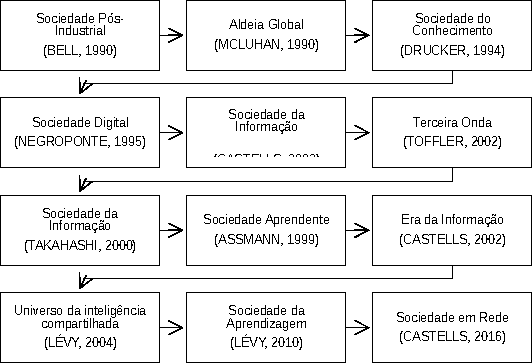
\includegraphics[width=\textwidth]{figura01.pdf}
  \caption{Definições para a sociedade.}
  \label{fig01}
  \source{Baseado em \textcite{silva2010}.}
\end{minipage}
\end{figure}

Todas essas definições, destacadas acima, retratavam pesquisas que
abordavam os impactos das TIC na sociedade. Ainda hoje, mesmo após todos
esses estudos, ainda se busca entender a atual cultura, marcada por
incontáveis transformações sociais, avanços tecnológicos e,
principalmente, influenciada pelo nascimento de uma nova sociedade que
se caracteriza pela chamada ``explosão informacional''
\cite{bell1990, gouveia2004a}. Portanto, para definir essa nova era de
intenso fluxo informacional, adotou-se, nesta dissertação, a
nomenclatura Sociedade da Informação (SI)\footnote{Sociedade da
  Informação é o conceito de uma organização geopolítica, que surgiu no
  início da terceira revolução industrial (fim do século XX), com o
  objetivo de utilizar da informação e das atuais tecnologias como
  recurso produtor de riqueza para desenvolvimento social e econômico
  \cite{castells2016}.}:

A Sociedade da informação está baseada nas tecnologias de informação e
comunicação que envolvem a aquisição, o armazenamento, o processamento e
a distribuição da informação por meios electrónicos, como a rádio, a
televisão, telefone e computadores, entre outros. Estas tecnologias não
transformam a sociedade por si só, mas são utilizadas pelas pessoas em
seus contextos sociais, económicos e políticos, criando uma nova
comunidade local e global: a Sociedade da Informação
\cite[p.~10]{gouveia2004a}.

A sociedade contemporânea passa por inúmeras mudanças com as atuais
tecnologias, o que levou estudiosos a defenderem a tese do nascimento de
um novo paradigma, o da Sociedade alicerçada na Informação, que surgiu
no final do século XX-- exatamente na década de 80 -- com a finalidade
de ser um fator-chave da forte ampliação e reorganização do capitalismo
\cite{morin2003, castells2016}.

Segundo \textcite[p.~78]{castells2016}, nós vivemos em uma nova sociedade, sem
fronteiras, um espaço global onde os indivíduos estão conectados em
redes, via internet, fruto da revolução tecnológica, da democratização e
forte utilização das TIC, no qual computadores e a telecomunicação têm
um papel importante nas mudanças sociais e culturais. \textcite{toffler2002}
chama esse momento de a ``Terceira Onda''\footnote{A primeira onda
  trata-se do surgimento da agricultura para o desenvolvimento social do
  homem; a segunda onda deu-se após a mecanização da agricultura pela
  revolução industrial; já a terceira onda surge no momento em que as
  TIC mudam o modo de viver em sociedade \cite{toffler2002}.} que,
apesar de ter iniciado no século XX, nos Estados Unidos da América,
desdobrou-se até os dias atuais, com o nascimento e fortalecimento de
uma nova civilização, a dos conectados, uma cultura em constante
mudança, baseada na informação.

Na SI, a informação é o elemento-chave que move e transforma a vida
social, cultural, política e econômica \cite{castells2016}. Ela se
constitui a partir de dois eixos centrais, a comunicação e a informação,
operacionalizados em dimensão global. Neste contexto, as redes físicas e
os sistemas inteligentes de comunicação e informação digital estão cada
vez mais desenvolvidos e sendo utilizados em todos os lugares, no
presencial e no virtual, de forma onipresente, pervasiva, infiltrada,
espalhada e difundida em escala global
\cite{takahashi2000, santaella2013}. Assim, essa sociedade tem como
particularidade o intenso trabalho no desenvolvimento das redes
informacionais e nos impactos sociais advindos da democratização e uso
das TIC \cite{castells2002, sorj2003}.

\textcite{castells2016}, para melhor esclarecer a SI, relata peculiaridades
deste novo momento em que se instaura um novo paradigma, o das TIC
\cite{freitas2015}, são elas:

\begin{enumerate}
\def\labelenumi{\alph{enumi})}
\item
  A informação é a base de tudo: em conjunto com a tecnologia, mantém
  uma relação associativa poderosa em que uma depende da
  outra. A partir dessa relação, as tecnologias são
  desenvolvidas para oferecer ao homem a possibilidade de
  atuar sobre a informação;
\item
  Os impactos das tecnologias repercutem fortemente na sociedade: as
  implicações das atuais tecnologias têm alta
  penetrabilidade  social, uma vez que a informação é o
  centro e parte integrante da  vida humana, seja ela
  individual ou coletiva, influenciando  principalmente na
  cultura, na economia e na política da sociedade;
\item
  A lógica de redes predomina sob a sociedade: destaca-se uma da
  característica primordial dessa nova sociedade. As
  tecnologias  favorecem a comunicação, a aproximação e a
  interação entre as  pessoas e, além disso, pode ser
  implementada em quaisquer  processos e relações
  pessoais;
\item
  Flexibilidade dos processos: as tecnologias permitem reconfigurar,
  alterar e reorganizar as informações, tornando todos os
  processos  gerados a partir dela reversíveis;
\item
  Convergências das tecnologias na atualidade: as tecnologias
  convergem e permeiam todos os setores da sociedade.
  Esse processo,  agora contínuo e em grande escala, faz
  com que todas as  informações, de diversos campos
  tecnológicos, sejam integradas e  acessadas por meio de
  categorias. Assim sendo, todos os indivíduos  vão poder
  atuar sobre a informação, exercendo um importante papel 
  na produção do conhecimento.
\end{enumerate}

Para \textcite[p.~10]{gouveia2004b}, as características da Sociedade podem
ser entendidas como ``{[}...{]} um entrelaçado de fluxos de informação a
que indivíduos e organizações têm que se readaptar {[}...{]}'',
detalhadas na \Cref{fig02}.

\begin{figure}[htbp]
\centering
\begin{minipage}{.5\textwidth} 
  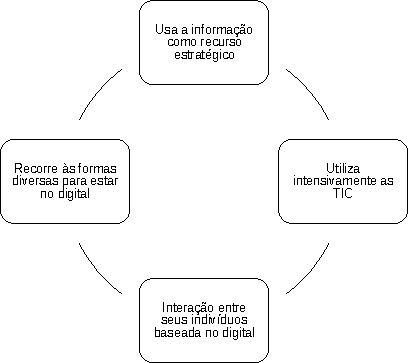
\includegraphics[width=\textwidth]{figura02.pdf}
  \caption{Características da Sociedade da Informação.}
  \label{fig02}
  \source{Baseada em \textcite{gouveia2004b}.}
\end{minipage}
\end{figure}

Ao analisar cada uma das características da SI representadas na \Cref{fig02},
observou-se a evidência dos impactos que as tecnologias produzem
na sociedade com o advento do processo de informatização e categorização
dos saberes \cite{freitas2015}. Percebeu-se que a SI é o ponto de
partida do processo que busca a democratização do saber e, a partir
dela, nascem novos ambientes para a busca e o compartilhar de
informações de forma ubíqua, sem barreiras de acesso às informações
\cite{levy2011, galvao2017}.

Ressaltou-se, neste estudo, não somente as tecnologias, mas também os
impactos gerados pelo uso dessas tecnologias e o nascimento de uma
cultura digital. Segundo \textcite{abreu2001}, essa nova cultura tem como
diretriz a desconstrução, renovação, criação, colaboração e interconexão
do saber. Essas diretrizes são como palavras de ordem do século XXI em
busca de uma inteligência coletiva \cite{coutinho2011}.

Assim sendo, a SI apresenta-se como um paradigma que nasce do processo
social de desenvolvimento científico e tecnológico, trazendo implicações
sociais, técnicas, culturais, econômicas e políticas, que se
reconfiguram, alteraram e reorganizam, modificando formas de pensar e
constituir a sociedade \cite{castells2016}. As TIC, nesse contexto, são
pensadas e inseridas em todos os setores sociais, de forma ubíqua, com o
objetivo de dinamizar e transformar a sociedade e a forma como nela se
vive \cite{abreu2001, silva2010}.

Diante das transformações provocadas pela pervasividade das TIC, as
formas de trabalhar, estudar, informar, pensar e comunicar na SI foram
se modificando com base na utilização da informação para produzir
conhecimentos. No campo da educação, por exemplo, a SI hoje se encarrega
de explorar todas as potencialidades das TIC e transmitir a informação a
fim de criar espaços para a aprendizagem democrática em que o acesso à
informação (matéria-prima), gerado e compartilhado em rede, esteja à
disponibilidade de todos \cite{santaella2013}.

Segundo \textcite{castells2016}, a informação, no contexto designado, tem o
papel de atuar como elemento que fomenta a criação de ambientes que
geram maior distribuição do conhecimento e oportunidade de aprendizagem
por meio das tecnologias. Com tais possibilidades, o processo de
aprendizagem é construído e outros modelos de ensino são reformulados,
caracterizando, assim, uma mudança sociocultural que altera as relações
sociais, os comportamentos e as formas de perceber e se comunicar com o
outro nesse universo informacional \cite{prensky2001}.

Constatou-se que, na SI, as informações transitam com ainda mais
velocidade, de maneira ubíqua, em diferentes espaços midiáticos, por
meio das TIC \cite{galvao2017}. Nesse processo de mudanças, percebeu-se
mais uma transição social. Desta vez, o nascimento da Sociedade da
Informação e Conhecimento (SIC), que se desenvolve em um contexto em que
as tecnologias e a comunicação se unem para fazer com que a informação
se torne matéria-prima da criação de espaços para uma série de
possibilidades a nível educacional, promovendo competências e
estimulando a aprendizagem, melhor explorados na seção seguinte
\cite{gomes2012}.



\section{Todos em busca do conhecimento}

Na SI, o conhecimento é a análise reflexiva de uma informação
transmitida por intermédio da experiência do indivíduo pelas TIC
\cite{castells2016}. E, dessa forma, a informação e o conhecimento
tornaram-se fontes de produtividade no atual contexto informacional
\cite{levy2011}. Com a informação e o conhecimento em mãos, os
indivíduos terão a capacidade de realizar a produção, o processo, a
aplicação, o compartilhamento da informação e transformá-la em
conhecimento \cite{takahashi2000}.

Todavia, é importante ressaltar que, apesar de haver uma relação
associativa entre ``informação'' e ``conhecimento'', \textcite{rezende2000}
%Rezende e Abreu (2000)
acentuam que os termos possuem algumas peculiaridades. Segundo os
autores,

\begin{quote}
Informação é todo o dado trabalhado, útil, tratado, com valor
significativo atribuído ou agregado a ele, e com um sentido natural e
lógico para quem usa a informação. O dado é entendido como um elemento
da informação, um conjunto de letras, números ou dígitos, que, tomado
isoladamente, não transmite nenhum conhecimento, ou seja, não contém um
significado claro. Quando a informação é ``trabalhada'' por pessoas e
pelos recursos computacionais, possibilitando a geração de cenários,
simulações e oportunidades, pode ser chamada de conhecimento. O conceito
de conhecimento complementa o de informação com valor relevante e de
propósito definido. \cite[p.~60]{abreu2001}.
\end{quote}

Ou seja, a construção do saber na SI resulta da relação entre a
informação e o conhecimento, fruto de um processo de criação. \textcite{levy2011}
enfatiza que, quando a informação é interpretada, pode acontecer
o processo de apropriação do conhecimento, que está embutida na
informação. Dá-se, então, a criação, o processo produtivo do saber. O
conhecimento nessa nova sociedade é consequência da aprendizagem, da
experiência do indivíduo com o acesso à informação por meio da
virtualidade. Todavia, esse processo não é linear. Não basta ter
informação para gerar conhecimento, é preciso saber o que fazer com ela
\cite{assmann1999, junqueiro2009, castells2016}.

Vale então trazer para esta discussão uma análise de \textcite[p.~88]{pellicer1997}
que, refletindo sobre os estudos de \textcite[p.~11]{ausubel1982},% Ausubel (1982, p.11),
acentua que,

\begin{quote}
As informações constituem a base do conhecimento, mas a aquisição deste
implica, antes de mais, o desencadear de uma série de operações
intelectuais, que colocam em relação os novos dados com as informações
armazenadas previamente pelo indivíduo. O conhecimento adquire-se, pois,
quando as diversas informações se interrelacionam mutuamente, criando
uma rede de significações que se interiorizam. Na actualidade, uma das
perturbações provocadas pelos médias é o facto de que o homem moderno
crê ter acesso à significação dos acontecimentos, simplesmente porque
recebeu informação sobre aqueles.
\end{quote}

Partindo do princípio de que é necessária a experiência para que o
conhecimento se torne concreto \cite{pellicer1997}, as informações em
rede passam por um processo de leitura reflexiva, obtenção de dados,
análise empírica e considerações sobre os dados. Esse processo, chamado
de divulgação científica\footnote{A divulgação científica é a divulgação
  dos resultados de uma pesquisa em diferentes formatos/meios de
  comunicação. Como troca de informações entre a comunidade científica e
  interessados pela divulgação - leigos ou não
  \cite{garvey1979, gomes2012}.}, é importante e fundamental para que a
informação seja transmitida e também assimilada \cite{mattelart2002}.

A divulgação científica permite que a pesquisa e seus resultados fiquem
de fácil acesso, em rede, para que toda comunidade tenha contato e
possa, a partir da pesquisa, ter conhecimento, poder de reflexão e
motivação para novas pesquisas e debates acerca da informação que se
investiga \cite{garvey1979, oliveira2017}. Nesse processo de pesquisa,
a comunicação é fundamental. \textcite{gomes2012} ressalta que, por meio da
comunicação, os indivíduos são capazes de realizar uma análise sobre a
produção científica divulgada e, assim, de certa forma, o conhecimento
passa por um processo de validação, sustentando a dinâmica da nova
economia informacional que se vive.

Nessa Sociedade, em que a informação é a matéria-prima, a divulgação
científica fez da ciência um saber cada vez mais público. Essa
popularização da ciência ocorre com o objetivo de despertar novos
talentos para dar sustentabilidade à própria ciência, fomentar o
nascimento de novos pesquisadores \cite{gomes2012}.

Buscou-se, então, mecanismos que agilizam o processo de leitura até a
fácil recuperação da informação do conhecimento produzido por meio de
uma ``memória'' (banco de dados) eficiente. Avaliando esse contexto, em
que a informação e as tecnologias juntas são capazes de promover o
conhecimento, a SIC ganha novas características, conforme \Cref{fig03}.


\begin{figure}[htbp]
\centering
\begin{minipage}{.75\textwidth} 
  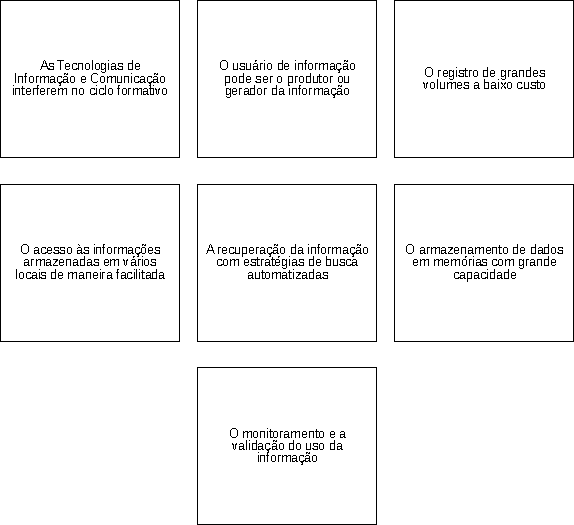
\includegraphics[width=\textwidth]{figura03.pdf}
  \caption{Características da Sociedade da Informação e Conhecimento.}
  \label{fig03}
  \source{Baseado em \textcite{castells2002}.}
\end{minipage}
\end{figure}


A SIC se configura na transmissão de informação em recursos que exploram
as potencialidades das TIC, bem como a criação de espaços de
aprendizagem e acesso ao conhecimento produzido e compartilhado na
internet pela rede de computadores \cite{castells2002,castells2016}. Nessa
sociedade, portanto, predominam a inovação tecnológica e avanço no
tratamento, armazenamento e transmissão da informação
\cite{webster2006, kenski2012}.

\textcite{takahashi2000} relata que, na SIC, o indivíduo é quem promove o
desenvolvimento da humanidade, mas que, para que esse desenvolvimento
ocorra, é necessário que ele seja detentor do saber, fator econômico
gerado a partir da informação, um bem comercial que permeia todos os
setores da sociedade.

Corroborando com este pensamento, \textcite{hargreaves2003} destaca a
importância que o indivíduo tem em saber explorar todas as
potencialidades das TIC, pois elas agregam valor à informação e promovem
melhor assimilação do conhecimento por meio da experiência em rede.

\textcite{takahashi2000,hargreaves2003} apontam, ainda, outra
característica para o contexto em que a sociedade explora as TIC em seu
benefício:

\begin{enumerate}
\def\labelenumi{\alph{enumi})}
\item
  Os fatores ``distância'' e ``tempo'' entre produtor de informação e
  usuário da informação não têm mais relevância, uma vez
  que os  indivíduos não precisam se deslocar, pois são as
  informações que  viajam, estão em todos os lugares e,
  por consequência, o  conhecimento também está ubíquo;
\item
  Se a informação, a comunicação e o conhecimento estão onipresentes,
  existe grande possibilidade de se descobrirem respostas
  inovadoras, cada vez mais críticas, de forma a dar
  sustentabilidade à ciência (saber);
\item
  As TIC levam o mundo real ao processo natural de convergência para o
  virtual \cite{levy2011} e transformam a SIC em uma
  verdadeira ``aldeia  global'' \cite{mcluhan1990};
\item
  As atuais tecnologias criam novas formas de conviver em sociedade e,
  com mudanças significativas nas relações sociais,
  surgem novos  modelos de trabalho, de fazer saúde,
  modelos de ensino, estilos de  aprendizagem (formal e
  informal), etc.
\end{enumerate}

No que tange aos novos modelos de ensino advindos com os impactos das
TIC, \textcite[p.~1]{siemens2004} relata que ``{[}...{]} a tecnologia
reorganizou o modo como vivemos, como nos comunicamos e como aprendemos
{[}...{]}'' e na SIC, a aprendizagem acontece de diferentes maneiras,
pensada para além da escola, numa perspectiva em que o saber pode ser
adquirido em múltiplas situações através de conexões na rede global.

Nesse contexto, o grande desafio das Instituições de Ensino do século
XXI é garantir a qualidade da construção do conhecimento em uma
sociedade em que as tecnologias ampliam todos os dias o acesso às
informações, gerando maior distribuição do conhecimento e oportunidade
de aprendizagem \cite{siemens2004,siemens2010}.

Em meio a esse processo, o papel do professor e do aluno também se
modifica. Para além de transmitir conhecimento, cabe ao professor neste
cenário ser um mediador na aprendizagem. Ao aluno, aprender competências
cognitivas para analisar, filtrar, avaliar e interpretar as informações
disponibilizadas na internet \cite{takahashi2000, coutinho2011}.

E, assim sendo, as TIC precisam ser inseridas no currículo educacional
para que possam colaborar no desenvolvimento da pedagogia da
virtualidade\footnote{Teoria crítica produzida na convergência das
  práticas educativas em rede e na apropriação do potencial emancipador
  da internet \cite{gomez2015}.}, propostas inovadoras para atuar com
as tecnologias educacionais no contexto das redes e da informação ubíqua
\cite{gomez2015, rojo2016}. A SIC proporciona aos indivíduos a
possibilidade de desenvolver o conhecimento por meio de processos
informais, que incluem o uso das TIC para mediar a construção do saber,
já que a informação está ubíqua e o conhecimento, por sua vez, também se
encontra por toda parte \cite{pozo2004}.

As propostas pedagógicas com uso de tecnologias tornam-se importantes
para que os alunos tenham uma boa atuação em diferentes atividades que
englobam os processos de aprendizagem multimídia. Todavia, \textcite{gomez2015}
enfatiza que o computador, a internet e os recursos da web devem mediar
as tarefas em sala de aula, mesclando com tarefas da educação
tradicional, e não serem utilizados como único instrumento.

Constatou-se que, com a globalização e a propagação da web
2.0\footnote{Termo utilizado para descrever a segunda geração da
  \emph{World Wide Web} (WWW), baseado no conceito de troca de
  informações e colaboração dos internautas com sites e serviços
  virtuais \cite{lambert2010}.}, surgiu a necessidade de aptidões, que
contemplassem os modernos processos midiáticos. Essas aptidões solicitam
novas propostas em sala de aula, que vão desde a reflexão sobre o uso
das tecnologias até experiências práticas condizentes com o mundo do
trabalho \cite{cherubin2012}. Essas novas propostas devem, portanto,
transformar o modelo de ensino que já não responde ao perfil da geração
de alunos cada vez mais conectados.

\textcite{rojo2016} entende que é necessário oferecer, à nova geração, o maior
número possível de recursos e estímulos, compreendidos em novas
metodologias e propostas didáticas na sala de aula. Diante dessa
afirmação, compreende-se, então, que as Instituições de Ensino têm o
papel importante de desenvolver práticas pedagógicas que façam uso
destes recursos de maneira criativa e eficaz nos processos de
aprendizagem.

As TIC na educação fizeram nascer múltiplos meios de interatividade, mas
para que os alunos estejam cada vez mais inseridos nesse processo de
aprendizagem por meio das atuais tecnologias, é necessário que a escola
dissemine a eles todas as possibilidades de interação oferecidas pela
cultura digital \cite{lisboa2010}.

As investigações acerca do uso de recursos multimidiáticos no processo
de aprendizagem apontam inúmeras contribuições das tecnologias na
formação do aluno em contextos de convergência \cite{pedro2002}.
\textcite{lisboa2010} ressaltam que, para além de
incentivar o uso de tecnologias para fins educacionais, os professores
devem apresentar propostas capazes de fazer com que os alunos possam
gerir com criticidade as informações e o conhecimento, uma vez que agora
eles se encontram por toda rede.




\section{Reflexões finais}

Este estudo apontou para um cenário em constante transformação, no qual
as TIC desempenham um papel central na reconfiguração social,
educacional e cultural. Contudo, muitas questões ainda estão em aberto,
e este não é um ponto de chegada, mas uma etapa de um processo contínuo
de reavaliação e adaptação. A transição da SI para a SIC parece
promissora, mas até que ponto esse avanço será realmente inclusivo? Até
que ponto as TIC podem se tornar, de fato, um meio democratizante, sem
perpetuar desigualdades ou criar novas formas de exclusão? Será que
todos os indivíduos estão de fato preparados para participar dessa nova
sociedade do conhecimento, ou apenas um seleto grupo será beneficiado?

As TIC, por mais que possibilitem a circulação de informações em uma
escala jamais vista, são também um terreno fértil para manipulações,
desinformação e desorganização social. A convergência das tecnologias e
a interconexão das redes globais oferecem, por um lado, a promessa de um
mundo mais colaborativo, mas por outro, surgem novas formas de controle
e vigilância, que merecem ser observadas com cautela. O que isso
significa para a privacidade, a liberdade individual e a própria noção
de pertencimento a uma sociedade?

O impacto das TIC na educação, por exemplo, abre um campo fértil para a
inovação pedagógica, mas também coloca em questão os métodos
tradicionais de ensino. O que acontece com o papel do professor quando
as informações estão amplamente disponíveis, mas ao mesmo tempo,
sobrecarregadas de complexidade? Como podemos garantir que a educação
seja verdadeiramente transformadora e não uma simples adaptação aos
recursos tecnológicos? Será que o conhecimento está sendo apenas
acessado de maneira rápida e superficial, sem que uma reflexão crítica
sobre ele seja suficientemente promovida?

A interação social também sofre profundas modificações, como o
enfraquecimento de formas tradicionais de comunicação e a emergência de
novas redes e relações. Mas, essa transformação é genuinamente positiva?
Estamos vivendo um processo de alienação, onde as interações virtuais
estão alterando as relações humanas mais profundas e complexas? Ou, ao
contrário, as TIC estão criando novas formas de proximidade e
coletividade, ampliando as possibilidades de se conectar com o outro?

A transição para a Sociedade do Conhecimento implica não apenas no
avanço das tecnologias, mas também na necessidade de uma reconfiguração
das práticas sociais, culturais e políticas. No entanto, até que ponto
as políticas públicas e as práticas educacionais estão acompanhando esse
movimento de forma eficaz? Existe uma visão crítica sobre como as TIC
estão sendo rompidas em diversos setores da sociedade, ou há um
incentivo cego ao seu uso sem considerar os possíveis efeitos
colaterais?

Este estudo não encerra as questões levantadas, mas sim, busca abrir um
leque de discussão. Como as TIC continuarão a reconfigurar as dinâmicas
de poder, os comportamentos e as práticas sociais? Qual será o papel das
futuras gerações nesse processo de transição contínua? Não sabemos as
respostas definitivas, mas é urgente que sigamos questionando,
refletindo e, acima de tudo, participando dessa transformação, a fim de
que as TIC cumpram seu papel de instrumento de emancipação, e não de
alienação.




\printbibliography\label{sec-bib}
% if the text is not in Portuguese, it might be necessary to use the code below instead to print the correct ABNT abbreviations [s.n.], [s.l.]
%\begin{portuguese}
%\printbibliography[title={Bibliography}]
%\end{portuguese}


%full list: conceptualization,datacuration,formalanalysis,funding,investigation,methodology,projadm,resources,software,supervision,validation,visualization,writing,review
\begin{contributors}[sec-contributors]
\authorcontribution{Jean Carlos da Silva Monteiro}[conceptualization,writing,review]
\authorcontribution{Luciano da Silva Façanha}[conceptualization,writing,review]
\end{contributors}

\end{document}

